\chapter{Projekt systemu (Michał Turski i Filip Jezierski)}
\label{chap:system_project}
Niniejszy rozdział przedstawia szczegółowy projekt systemu aplikacji webowej \textbf{UniGuesser}. Opisane zostaną kluczowe elementy architektury systemu, w tym warstwy aplikacji, baza danych oraz najbardziej kluczowe interakcje użytkownika z systemem. Zaczynając od ogólnego przeglądu architektury, przejdziemy do szczegółowego omówienia poszczególnych komponentów i ich wzajemnych relacji.

W aplikacji zastosowano architekturę warstwową, której szczegółowa implementacja zostanie opisana w niniejszym rozdziale. Na najwyższym poziomie abstrakcji system można podzielić na trzy główne warstwy: warstwę prezentacji (frontend), warstwę logiki biznesowej (backend) oraz warstwę persystencji danych (baza danych). Podział ten odzwierciedla sposób izolowania odpowiedzialności poszczególnych komponentów. Dzięki temu użytkownik komunikuje się z aplikacją poprzez interfejs użytkownika, który następnie przekazuje żądania do warstwy logiki biznesowej. Ta z kolei przetwarza żądania, wykonuje odpowiednie operacje i komunikuje się z bazą danych w celu przechowywania lub pobierania danych.

\begin{figure}[h]
    \centering
    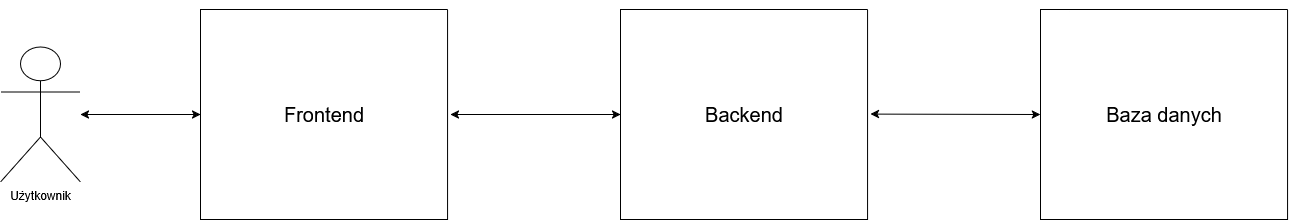
\includegraphics[width=1.0\textwidth]{./images/architecture-overview.png}
    \caption{Uproszczony schemat architektury systemu UniGuesser – ogólny podział na warstwy}
    \label{fig:architecture-overview}
\end{figure}


\section{Architektura logiki biznesowej (Michał Turski)}
Architektura w aplikacji \textbf{UniGuesser} została zbudowana w oparciu o Command-Query Responsibility Segregation (CQRS) oraz Domain-Driven Design (DDD), które
są obecnie standardem w wytwarzaniu oprogramowania. [dodać źródło na potwierdznie słów]
Ponadto zdecydowaliśmy na wybór architektury monolitycznej ze względu na szybkość rozwoju i łatwość wdrożenia, co pomogło skupić się nam na aspekcie funkcjonalnym aplikacji w początkowej fazie jej tworzenia.

\subsection{Wzorzec CQRS (Command Query Responsibility Segregation)}
Wykorzystany został również wzorzec CQRS. Zakłada on rozdzielenie operacji modyfikujących stan systemu (komendy) od operacji, które odczytują dane (zapytania). Pozwala to na lepsze skalowanie i rozdzielenie logiki aplikacji. Dzięki temu można optymalizować każdą z tych operacji niezależnie, co przekłada się na wydajność i czytelność kodu. W kontekście skalowalności systemu zastosowano uproszczoną implementację wzorca CQRS z pojedynczą bazą danych, która jest wystarczająca przy przewidywanym obciążeniu nieprzekraczającym 50 zapytań na sekundę. Taka architektura zapewnia odpowiednią wydajność przy jednoczesnym zachowaniu prostoty infrastruktury.

\begin{figure}[h]
    \centering
    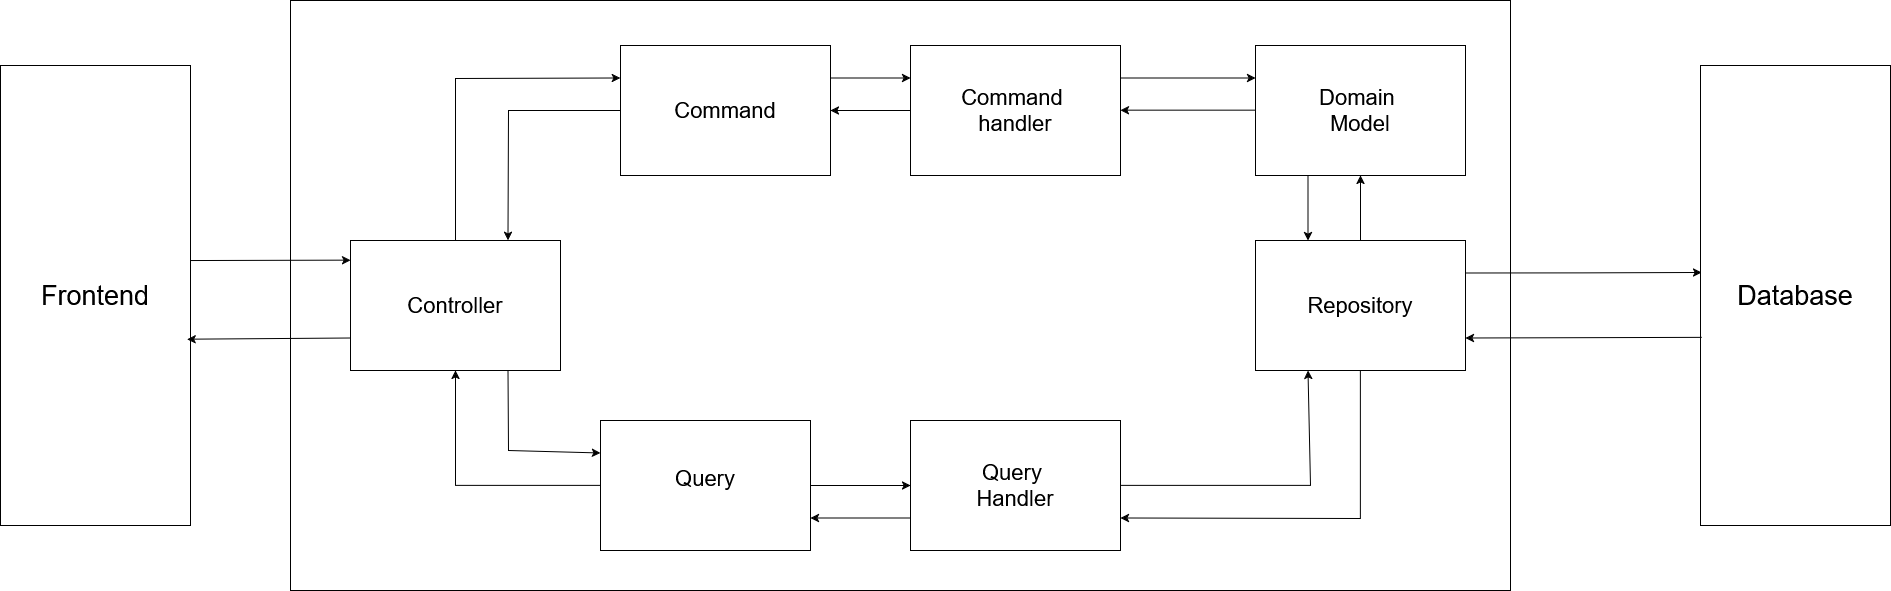
\includegraphics[width=1.0\textwidth]{./images/cqrs-communication.png}
    \caption{Schemat komunikacji przy zastosowaniu wzorca CQRS}
    \label{fig:cqrs-communication}
\end{figure}



\subsection{Zastosowanie DDD (Domain-Driven Design)}
Model systemu został zaprojektowany zgodnie z podejściem Domain-Driven Design (DDD), które kładzie nacisk na zrozumienie i modelowanie domeny problemowej. W aplikacji definiujemy trzy główne warstwy DDD: warstwę domeny, warstwę aplikacji oraz warstwę infrastruktury. Każda z warstw znajduje się w osobnym module, co ułatwia zarządzanie kodem i jego rozwój. Dodatkowo w aplikacji wydzielony został czwarty moduł „API”, który odpowiada za komunikację z warstwą prezentacji, co zmniejsza złożoność warstwy aplikacji. Moduł „API” obsługuje zarówno zapytania, jak i komendy, delegując je odpowiednio do warstwy aplikacji, która następnie komunikuje się z warstwą domeny i infrastruktury w celu realizacji żądanych operacji.

\section{Baza danych (Michał Turski)}

W aplikacji zastosowano relacyjną bazę danych, do przechowywania informacji o aktualnych i przeszłych sesjach gier, użytkownikach, lokalizacjach oraz wynikach. Zdecydowaliśmy się na wykorzystanie relacyjnej bazy danych ze względu na duża ilość powiąza między encjami oraz potrzebę zapewnienia integralności danych między nimi. Relacyjne bazy danych zapewniaja ACID (Atomicity, Consistency, Isolation, Durability), co jest kluczowe dla zachowania spójności danych w rozgrywce. 

\subsection{Diagram ERD}
Przedstawiony na rysunku \ref{fig:erd-diagram} diagram ERD (Entity-Relationship Diagram) ilustruje strukturę bazy danych aplikacji UniGuesser, pokazując główne tabele oraz relacje między nimi. Użytkownik może posiadać wiele sesji gier, a każda sesja ma określoną liczbę rund, z których każda posiada przypisaną do siebie lokacje. Ponadto każde miejsce może mieć swojego autora (użytkownika), który dodał je do bazy danych. 

\begin{figure}[h]
    \centering
    
\includegraphics[width=1.0\textwidth]{./images/erdDiagram.png}
    \caption{Diagram ERD (Entity-Relationship Diagram) dla bazy danych aplikacji UniGuesser}
    \label{fig:erd-diagram}
\end{figure}

\subsection{Opis głównych tabel i związków}

\begin{itemize}
    \item \textbf{Users (Użytkownicy)} – tabela przechowująca informacje o użytkownikach aplikacji.
\end{itemize}

\begin{table}[H]
\centering
\renewcommand{\arraystretch}{1.2}
\begin{tabular}{|p{2.5cm}|p{8cm}|p{2.5cm}|}
\hline
\textbf{Atrybut} & \textbf{Opis} & \textbf{Typ / Uwagi} \\ \hline
ID & Unikalny identyfikator użytkownika. & Klucz główny \\ \hline
Nickname & Unikalna nazwa użytkownika. & Tekst \\ \hline
Email & Unikalny adres e-mail użytkownika. & Tekst \\ \hline
PasswordHash & Zaszyfrowane hasło użytkownika. & Tekst \\ \hline
CreatedAt & Data i czas utworzenia konta. & Data/Czas \\ \hline
Role & Rola użytkownika w systemie (np. użytkownik, administrator). & Enumeracja \\ \hline
\end{tabular}
\caption{Tabela \texttt{Users}}

\end{table}

\textbf{GameSessions (Sesje gier)} – tabela przechowująca informacje o aktywnych i zakończonych rozgrywkach.

\begin{table}[H]
\centering
\renewcommand{\arraystretch}{1.2}
\begin{tabular}{|p{2.8cm}|p{8.5cm}|p{2cm}|}
\hline
\textbf{Atrybut} & \textbf{Opis} & \textbf{Typ / Uwagi} \\ \hline
ID & Unikalny identyfikator sesji gry. & Klucz główny \\ \hline
GameMode & Tryb gry w danej sesji. & Enumeracja \\ \hline
GameEndDate & Data, do której rozgrywka jest aktywna. & Data/Czas \\ \hline
RoundNumber & Aktualnie rozgrywana runda. & Liczba \\ \hline
GameScore & Łączna liczba punktów zdobytych. & Liczba całkowita \\ \hline
Difficulty & Poziom trudności sesji. & Enumeracja \\ \hline
FinishedTime & Data zakończenia rozgrywki. & Data/Czas \\ \hline
UserID & Identyfikator użytkownika. & Klucz obcy → Users \\ \hline
\end{tabular}
\caption{Tabela \texttt{GameSessions}}
\label{tab:game-sessions}
\end{table}

\textbf{Rounds (Rundy)} – tabela przechowująca informacje o poszczególnych rundach w sesji gry.

\begin{table}[H]
\centering
\renewcommand{\arraystretch}{1.2}
\begin{tabular}{|p{3cm}|p{8.5cm}|p{1.8cm}|}
\hline
\textbf{Atrybut} & \textbf{Opis} & \textbf{Typ / Uwagi} \\ \hline
ID & Unikalny identyfikator rundy. & Klucz główny \\ \hline
GuessedLatitude & Szerokość geograficzna wskazana przez użytkownika. & Liczba zmiennoprzecinkowa \\ \hline
GuessedLongitude & Długość geograficzna wskazana przez użytkownika. & Liczba zmiennoprzecinkowa \\ \hline
Score & Punkty zdobyte w rundzie. & Liczba całkowita \\ \hline
GameSessionID & Identyfikator sesji gry. & Klucz obcy → GameSessions \\ \hline
LocationID & Identyfikator lokacji. & Klucz obcy → Places \\ \hline
\end{tabular}
\caption{Tabela \texttt{Rounds}} 
\label{tab:rounds}
\end{table}

\textbf{Places (Lokacje)} – tabela przechowująca informacje o lokacjach dostępnych w grze.

\begin{table}[H]
\centering
\renewcommand{\arraystretch}{1.2}
\begin{tabular}{|p{2.5cm}|p{8cm}|p{2.5cm}|}
\hline
\textbf{Atrybut} & \textbf{Opis} & \textbf{Typ / Uwagi} \\ \hline
ID & Unikalny identyfikator lokacji. & Klucz główny \\ \hline
Name & Nazwa lokacji. & Tekst \\ \hline
Description & Opis lokacji. & Tekst \\ \hline
Latitude & Szerokość geograficzna lokacji. & Liczba zmiennoprzecinkowa \\ \hline
Longitude & Długość geograficzna lokacji. & Liczba zmiennoprzecinkowa \\ \hline
Difficulty & Poziom trudności lokacji. & Enumeracja \\ \hline
ImageUrl & Adres URL obrazu lokacji. & Tekst \\ \hline
AltImage & Tekst alternatywny dla obrazu lokacji. & Tekst \\ \hline
CreationTime & Data i czas dodania lokacji. & Data/Czas \\ \hline
AuthorID & Identyfikator autora lokacji. & Klucz obcy → Users \\ \hline
\end{tabular}
\caption{Tabela \texttt{Places}}
\end{table}

\section{Analiza interakcji użytkownika z systemem (Michał Turski)}
W rozdziale przedstawione zostaną możliwości i przebieg kluczowych funkcjonalności aplikacji UniGuesser z perspektywy użytkownika końcowego. Opisane zostaną główne przypadki użycia oraz interakcje między użytkownikiem a systemem podczas typowej rozgrywki.

\subsection{Przypadki użycia aplikacji}
Przedstawiony na rysunku \ref{fig:use-case-diagram} diagram przypadków użycia ilustruje główne funkcjonalności aplikacji UniGuesser z perspektywy użytkownika moderatora i administratora. Użytkownik może rejestrować się i logować do systemu, rozpoczynać nowe sesje gier, uczestniczyć w rozgrywkach, przeglądać wyniki innych użytkowników, oraz proponować nowe lokacje. Moderator dodatkowo może zatwierdzać lub odrzucać proponowane lokacje, natomiast administrator ma uprawnienia do zarządzania użytkownikami.

\begin{figure}[H]
    \centering
    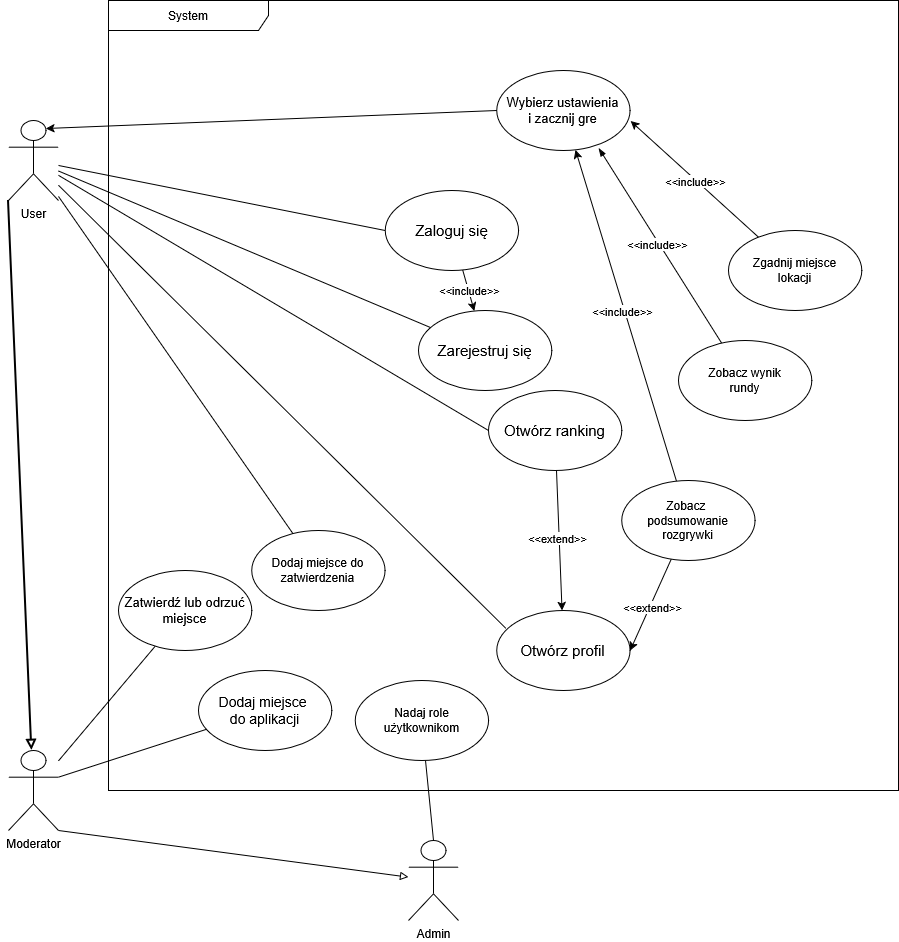
\includegraphics[width=1.0\textwidth]{./images/useCaseDiagram.png}
    \caption{Diagram przypadków użycia aplikacji UniGuesser}
    \label{fig:use-case-diagram}
\end{figure}

\subsection{Diagram sekwencji rozgrywki}

Diagram sekwencji przedstawiony na rysunku \ref{fig:sequence-diagram} ilustruje przebieg interakcji między użytkownikiem a systemem podczas typowej rozgrywki w aplikacji UniGuesser. Proces rozpoczyna się od momentu, gdy użytkownik uruchamia nową grę, poprzez kolejne rundy, aż do momentu zakończenia sesji i wyświetlenia wyników końcowych.

\begin{figure}[H]
    \centering
    \makebox[\textwidth]{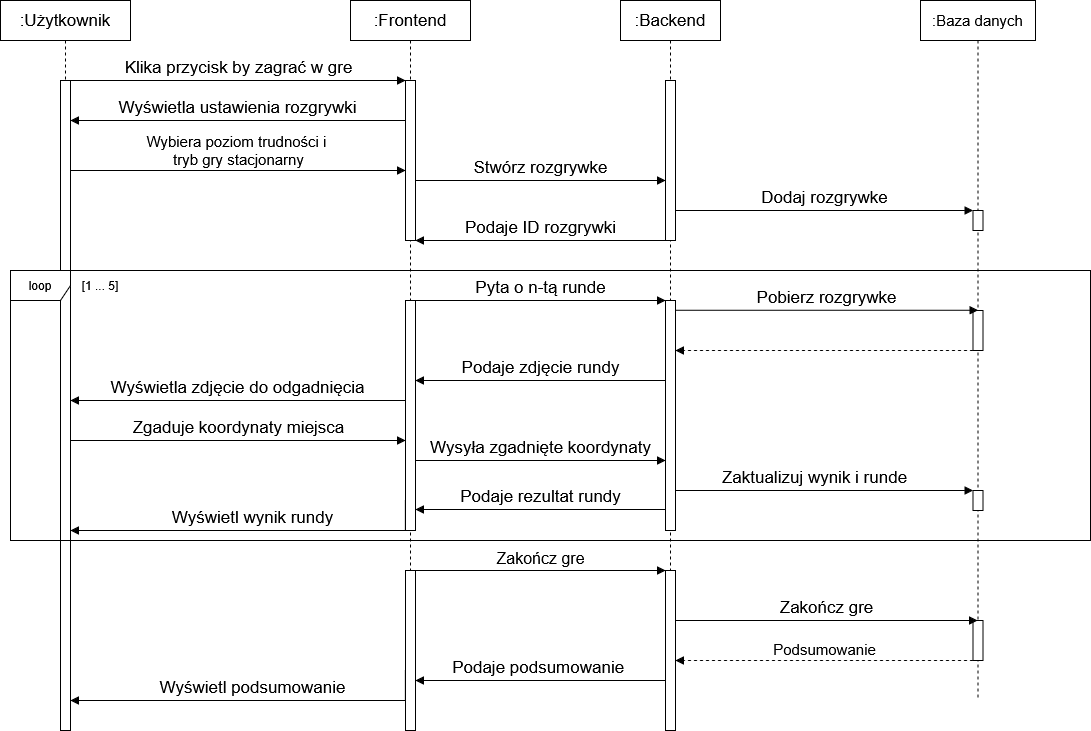
\includegraphics[width=1.2\textwidth]{./images/standardGameplaySequenceDiagram.png}}
    \caption{Diagram sekwencji przedstawiający przebieg rozgrywki w aplikacji UniGuesser}
    \label{fig:sequence-diagram}
\end{figure}

\section{Estetyka i design (Filip Jezierski) }
Wygląd aplikacji został zaprojektowany z myślą o prostocie, intuicyjności oraz atrakcyjności wizualnej. Poniżej przedstawiono kluczowe elementy designu interfejsu użytkownika.

\subsection{Ogólny projekt interfejsu}
Design interfejsu użytkownika naszej aplikacji skupia się na minimalizmie i czytelności. Stosowane są przyjęte jako standardowe układy elementów, takie jak menu nawigacji w górnej części ekranu, co ułatwia poruszanie się po aplikacji, nawet dla nowych użytkowników. Podstrony są zaprojektowane tak, aby unikać nadmiaru informacji, co pozwala użytkownikom skupić się na kluczowych funkcjonalnościach. W trakcie rozgrywki centralnym elementem interfejsu jest interaktywna mapa, która umożliwia użytkownikom łatwe wskazywanie lokalizacji, a pozostałe elementy interfejsu są rozmieszczone w sposób intuicyjny wokół niej.

\subsection{Kolorystyka}
% todo: screen z aplikacji
Aplikacja wykorzystuje dwukolorową paletę barw, opartą na odcieniach białego i ciemnoniebieskiego, inspirowaną kolorystyką Politechniki Gdańskiej. Biały kolor dominuje w tle, co zapewnia czystość i przejrzystość interfejsu, natomiast niebieskie akcenty są używane do wyróżnienia kluczowych elementów, takich jak przyciski, nagłówki czy linki. Przykładowe zastosowanie palety kolorów przedstawia rysunek \ref{fig:register-form}. Taka kolorystyka zapewnia odpowiedni kontrast i ułatwia czytelność tekstu, zwłaszcza przy korzystaniu z aplikacji w różnych warunkach oświetleniowych, co jest szczególnie istotne ze względu na terenowy charakter gry.

\begin{figure}[H]
    \centering
    \makebox[\textwidth]{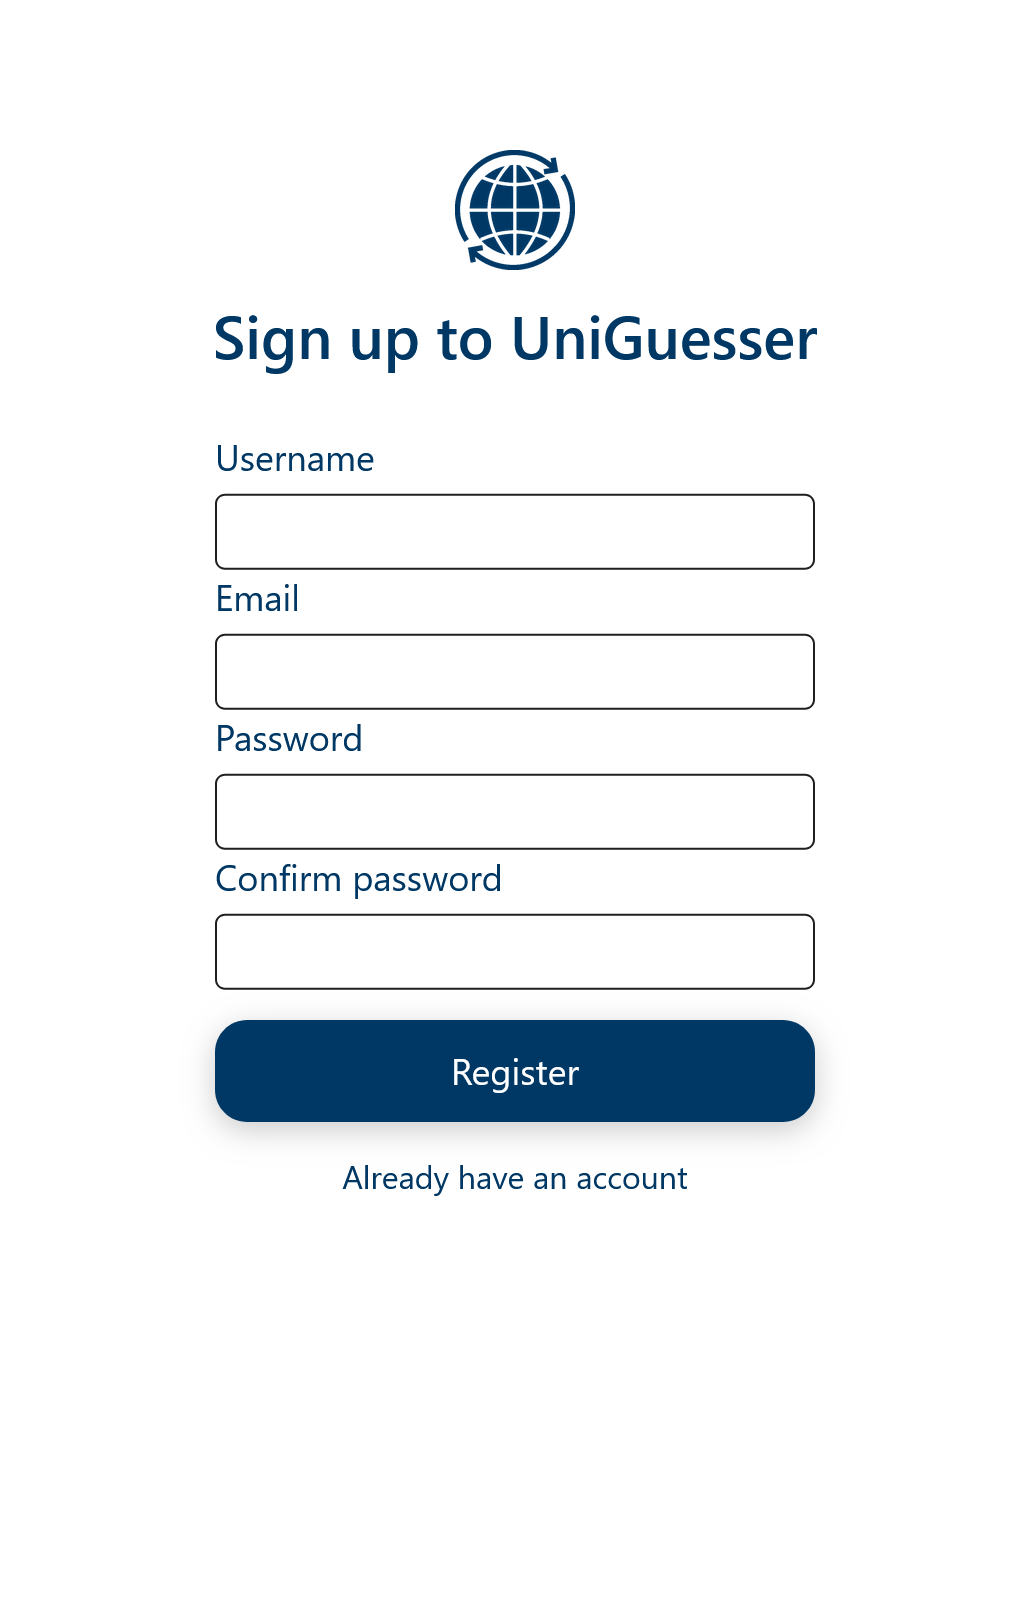
\includegraphics[width=0.5\textwidth]{./images/registerForm.png}}
    \caption{Przykładowy ekran rejestracji użytkownika w aplikacji UniGuesser, ilustrujący zastosowaną kolorystykę}
    \label{fig:register-form}
\end{figure}

\subsection{Typografia}
Aplikacja wykorzystuje czcionkę Roboto, która jest nowoczesna, czytelna i estetyczna. Czcionka ta jest szeroko stosowana w projektach webowych ze względu na swoją uniwersalność i dobrą czytelność na ekranach o różnych rozdzielczościach.

\subsection{Ikony}
W interfejsie użytkownika wykorzystano zestaw prostych i intuicyjnych ikon, pochodzących z biblioteki Google Icons. Ikony te są spójne stylistycznie i pomagają użytkownikom szybko zidentyfikować funkcje oraz akcje dostępne w aplikacji. Dzięki zastosowaniu powszechnie rozpoznawalnych symboli, nawigacja staje się bardziej intuicyjna, co przekłada się na lepsze doświadczenie użytkownika.

\subsection{Responsywność}
Aplikacja została zaprojektowana z myślą o responsywności, co oznacza, że dostosowuje się do różnych rozmiarów ekranów i urządzeń. Dzięki temu użytkownicy mogą korzystać z aplikacji zarówno na komputerach stacjonarnych, jak i urządzeniach mobilnych, bez utraty funkcjonalności czy estetyki. Elementy interfejsu, takie jak przyciski, formularze czy mapy, automatycznie dostosowują swoje rozmiary i układ w zależności od dostępnej przestrzeni ekranowej. Na mniejszych ekranach, takich jak smartfony, menu nawigacyjne jest ukryte za ikoną hamburgera, co pozwala zaoszczędzić miejsce i utrzymać przejrzystość interfejsu. Ponadto, kluczowe funkcje pozostają łatwo dostępne, a tekst i grafiki są skalowane odpowiednio do rozdzielczości ekranu, zapewniając optymalne doświadczenie użytkownika niezależnie od urządzenia.

\chapter{Projekt systemu (Michał Turski i Filip Jezierski)}
\label{chap:system_project}
Niniejszy rozdział przedstawia szczegółowy projekt systemu aplikacji webowej \textbf{UniGuesser}. Opisane zostaną kluczowe elementy architektury systemu, w tym warstwy aplikacji, baza danych oraz najbardziej kluczowe interakcje użytkownika z systemem. Zaczynając od ogólnego przeglądu architektury, przejdziemy do szczegółowego omówienia poszczególnych komponentów i ich wzajemnych relacji.

W aplikacji zastosowano architekturę warstwową, której szczegółowa implementacja zostanie opisana w niniejszym rozdziale. Na najwyższym poziomie abstrakcji system można podzielić na trzy główne warstwy: warstwę prezentacji (frontend), warstwę logiki biznesowej (backend) oraz warstwę persystencji danych (baza danych). Podział ten odzwierciedla sposób izolowania odpowiedzialności poszczególnych komponentów. Dzięki temu użytkownik komunikuje się z aplikacją poprzez interfejs użytkownika, który następnie przekazuje żądania do warstwy logiki biznesowej. Ta z kolei przetwarza żądania, wykonuje odpowiednie operacje i komunikuje się z bazą danych w celu przechowywania lub pobierania danych.

\begin{figure}[h]
    \centering
    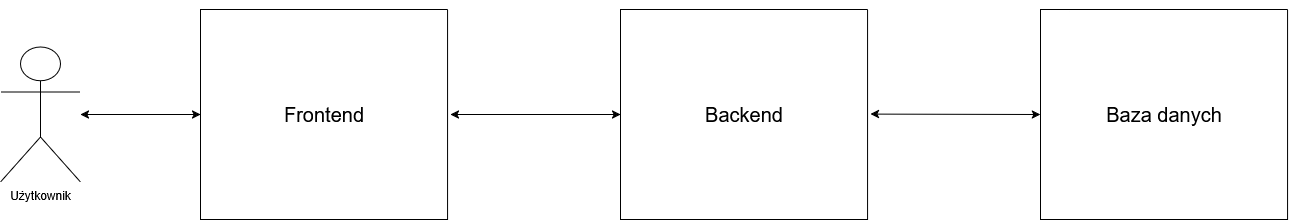
\includegraphics[width=1.0\textwidth]{./images/architecture-overview.png}
    \caption{Uproszczony schemat architektury systemu UniGuesser – ogólny podział na warstwy}
    \label{fig:architecture-overview}
\end{figure}


\section{Architektura logiki biznesowej (Michał Turski)}
Architektura w aplikacji \textbf{UniGuesser} została zbudowana w oparciu o Command-Query Responsibility Segregation (CQRS) oraz Domain-Driven Design (DDD), które
są obecnie standardem w wytwarzaniu oprogramowania. [dodać źródło na potwierdznie słów]
Ponadto zdecydowaliśmy na wybór architektury monolitycznej ze względu na szybkość rozwoju i łatwość wdrożenia, co pomogło skupić się nam na aspekcie funkcjonalnym aplikacji w początkowej fazie jej tworzenia.

\subsection{Wzorzec CQRS (Command Query Responsibility Segregation)}
Wykorzystany został również wzorzec CQRS. Zakłada on rozdzielenie operacji modyfikujących stan systemu (komendy) od operacji, które odczytują dane (zapytania). Pozwala to na lepsze skalowanie i rozdzielenie logiki aplikacji. Dzięki temu można optymalizować każdą z tych operacji niezależnie, co przekłada się na wydajność i czytelność kodu. W kontekście skalowalności systemu zastosowano uproszczoną implementację wzorca CQRS z pojedynczą bazą danych, która jest wystarczająca przy przewidywanym obciążeniu nieprzekraczającym 50 zapytań na sekundę. Taka architektura zapewnia odpowiednią wydajność przy jednoczesnym zachowaniu prostoty infrastruktury.

\begin{figure}[h]
    \centering
    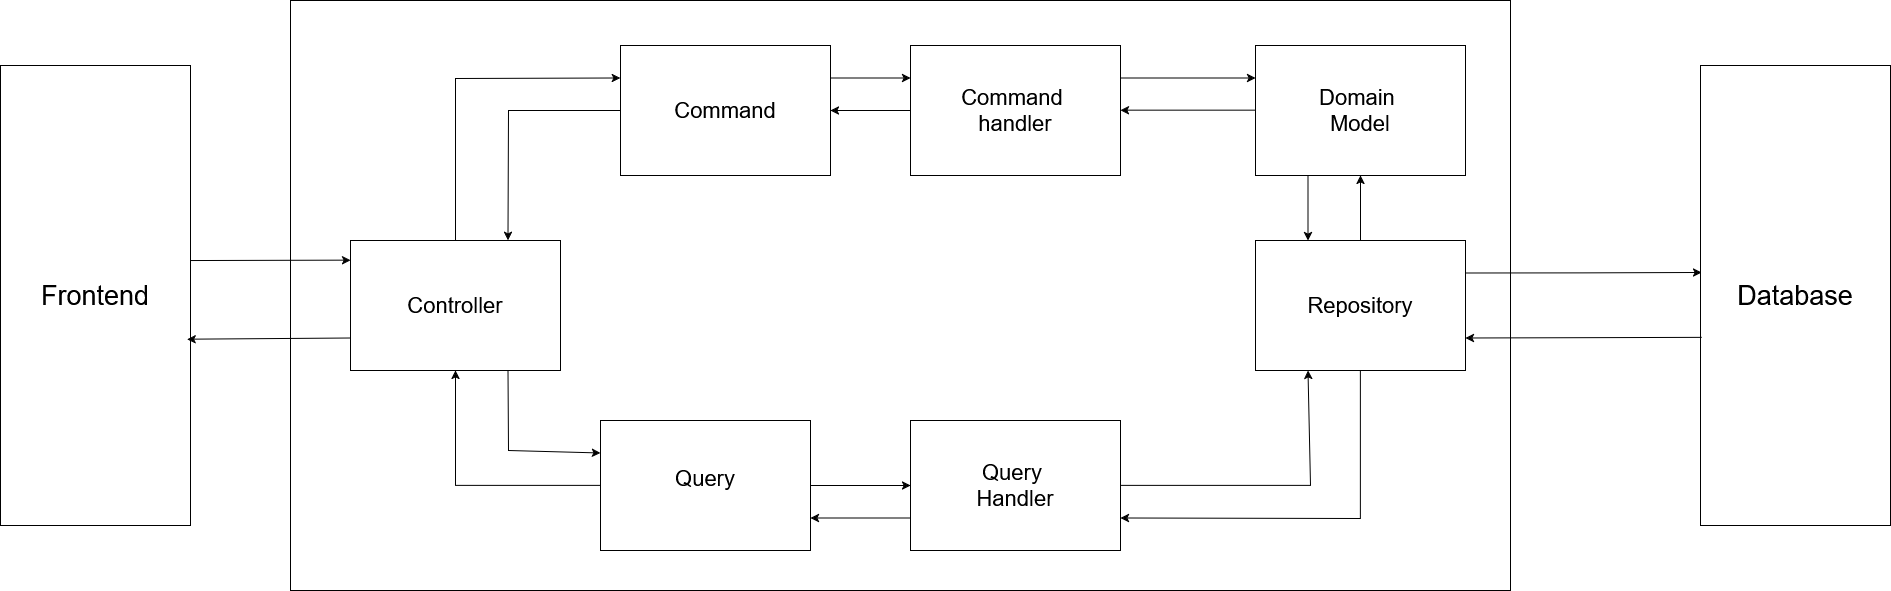
\includegraphics[width=1.0\textwidth]{./images/cqrs-communication.png}
    \caption{Schemat komunikacji przy zastosowaniu wzorca CQRS}
    \label{fig:cqrs-communication}
\end{figure}



\subsection{Zastosowanie DDD (Domain-Driven Design)}
Model systemu został zaprojektowany zgodnie z podejściem Domain-Driven Design (DDD), które kładzie nacisk na zrozumienie i modelowanie domeny problemowej. W aplikacji definiujemy trzy główne warstwy DDD: warstwę domeny, warstwę aplikacji oraz warstwę infrastruktury. Każda z warstw znajduje się w osobnym module, co ułatwia zarządzanie kodem i jego rozwój. Dodatkowo w aplikacji wydzielony został czwarty moduł „API”, który odpowiada za komunikację z warstwą prezentacji, co zmniejsza złożoność warstwy aplikacji. Moduł „API” obsługuje zarówno zapytania, jak i komendy, delegując je odpowiednio do warstwy aplikacji, która następnie komunikuje się z warstwą domeny i infrastruktury w celu realizacji żądanych operacji.

\section{Baza danych (Michał Turski)}

W aplikacji zastosowano relacyjną bazę danych, do przechowywania informacji o aktualnych i przeszłych sesjach gier, użytkownikach, lokalizacjach oraz wynikach. Zdecydowaliśmy się na wykorzystanie relacyjnej bazy danych ze względu na duża ilość powiąza między encjami oraz potrzebę zapewnienia integralności danych między nimi. Relacyjne bazy danych zapewniaja ACID (Atomicity, Consistency, Isolation, Durability), co jest kluczowe dla zachowania spójności danych w rozgrywce. 

\subsection{Diagram ERD}
Przedstawiony na rysunku \ref{fig:erd-diagram} diagram ERD (Entity-Relationship Diagram) ilustruje strukturę bazy danych aplikacji UniGuesser, pokazując główne tabele oraz relacje między nimi. Użytkownik może posiadać wiele sesji gier, a każda sesja ma określoną liczbę rund, z których każda posiada przypisaną do siebie lokacje. Ponadto każde miejsce może mieć swojego autora (użytkownika), który dodał je do bazy danych. 

\begin{figure}[h]
    \centering
    
\includegraphics[width=1.0\textwidth]{./images/erdDiagram.png}
    \caption{Diagram ERD (Entity-Relationship Diagram) dla bazy danych aplikacji UniGuesser}
    \label{fig:erd-diagram}
\end{figure}

\subsection{Opis głównych tabel i związków}

\begin{itemize}
    \item \textbf{Users (Użytkownicy)} – tabela przechowująca informacje o użytkownikach aplikacji.
\end{itemize}

\begin{table}[H]
\centering
\renewcommand{\arraystretch}{1.2}
\begin{tabular}{|p{2.5cm}|p{8cm}|p{2.5cm}|}
\hline
\textbf{Atrybut} & \textbf{Opis} & \textbf{Typ / Uwagi} \\ \hline
ID & Unikalny identyfikator użytkownika. & Klucz główny \\ \hline
Nickname & Unikalna nazwa użytkownika. & Tekst \\ \hline
Email & Unikalny adres e-mail użytkownika. & Tekst \\ \hline
PasswordHash & Zaszyfrowane hasło użytkownika. & Tekst \\ \hline
CreatedAt & Data i czas utworzenia konta. & Data/Czas \\ \hline
Role & Rola użytkownika w systemie (np. użytkownik, administrator). & Enumeracja \\ \hline
\end{tabular}
\caption{Tabela \texttt{Users}}
\end{table}

\textbf{GameSessions (Sesje gier)} – tabela przechowująca informacje o aktywnych i zakończonych rozgrywkach.

\begin{table}[H]
\centering
\renewcommand{\arraystretch}{1.2}
\begin{tabular}{|p{2.8cm}|p{8.5cm}|p{2cm}|}
\hline
\textbf{Atrybut} & \textbf{Opis} & \textbf{Typ / Uwagi} \\ \hline
ID & Unikalny identyfikator sesji gry. & Klucz główny \\ \hline
GameMode & Tryb gry w danej sesji. & Enumeracja \\ \hline
GameEndDate & Data, do której rozgrywka jest aktywna. & Data/Czas \\ \hline
RoundNumber & Aktualnie rozgrywana runda. & Liczba \\ \hline
GameScore & Łączna liczba punktów zdobytych. & Liczba całkowita \\ \hline
Difficulty & Poziom trudności sesji. & Enumeracja \\ \hline
FinishedTime & Data zakończenia rozgrywki. & Data/Czas \\ \hline
UserID & Identyfikator użytkownika. & Klucz obcy → Users \\ \hline
\end{tabular}
\caption{Tabela \texttt{GameSessions}}
\end{table}

\textbf{Rounds (Rundy)} – tabela przechowująca informacje o poszczególnych rundach w sesji gry.

\begin{table}[H]
\centering
\renewcommand{\arraystretch}{1.2}
\begin{tabular}{|p{3cm}|p{8.5cm}|p{1.8cm}|}
\hline
\textbf{Atrybut} & \textbf{Opis} & \textbf{Typ / Uwagi} \\ \hline
ID & Unikalny identyfikator rundy. & Klucz główny \\ \hline
GuessedLatitude & Szerokość geograficzna wskazana przez użytkownika. & Liczba zmiennoprzecinkowa \\ \hline
GuessedLongitude & Długość geograficzna wskazana przez użytkownika. & Liczba zmiennoprzecinkowa \\ \hline
Score & Punkty zdobyte w rundzie. & Liczba całkowita \\ \hline
GameSessionID & Identyfikator sesji gry. & Klucz obcy → GameSessions \\ \hline
LocationID & Identyfikator lokacji. & Klucz obcy → Places \\ \hline
\end{tabular}
\caption{Tabela \texttt{Rounds}}
\end{table}

\textbf{Places (Lokacje)} – tabela przechowująca informacje o lokacjach dostępnych w grze.

\begin{table}[H]
\centering
\renewcommand{\arraystretch}{1.2}
\begin{tabular}{|p{2.5cm}|p{8cm}|p{2.5cm}|}
\hline
\textbf{Atrybut} & \textbf{Opis} & \textbf{Typ / Uwagi} \\ \hline
ID & Unikalny identyfikator lokacji. & Klucz główny \\ \hline
Name & Nazwa lokacji. & Tekst \\ \hline
Description & Opis lokacji. & Tekst \\ \hline
Latitude & Szerokość geograficzna lokacji. & Liczba zmiennoprzecinkowa \\ \hline
Longitude & Długość geograficzna lokacji. & Liczba zmiennoprzecinkowa \\ \hline
Difficulty & Poziom trudności lokacji. & Enumeracja \\ \hline
ImageUrl & Adres URL obrazu lokacji. & Tekst \\ \hline
AltImage & Tekst alternatywny dla obrazu lokacji. & Tekst \\ \hline
CreationTime & Data i czas dodania lokacji. & Data/Czas \\ \hline
AuthorID & Identyfikator autora lokacji. & Klucz obcy → Users \\ \hline
\end{tabular}
\caption{Tabela \texttt{Places}}
\end{table}

\section{Analiza interakcji użytkownika z systemem (Michał Turski)}
W rozdziale przedstawione zostaną możliwości i przebieg kluczowych funkcjonalności aplikacji UniGuesser z perspektywy użytkownika końcowego. Opisane zostaną główne przypadki użycia oraz interakcje między użytkownikiem a systemem podczas typowej rozgrywki.

\subsection{Przypadki użycia aplikacji}
Przedstawiony na rysunku \ref{fig:use-case-diagram} diagram przypadków użycia ilustruje główne funkcjonalności aplikacji UniGuesser z perspektywy użytkownika moderatora i administratora. Użytkownik może rejestrować się i logować do systemu, rozpoczynać nowe sesje gier, uczestniczyć w rozgrywkach, przeglądać wyniki innych użytkowników, oraz proponować nowe lokacje. Moderator dodatkowo może zatwierdzać lub odrzucać proponowane lokacje, natomiast administrator ma uprawnienia do zarządzania użytkownikami.

\begin{figure}[H]
    \centering
    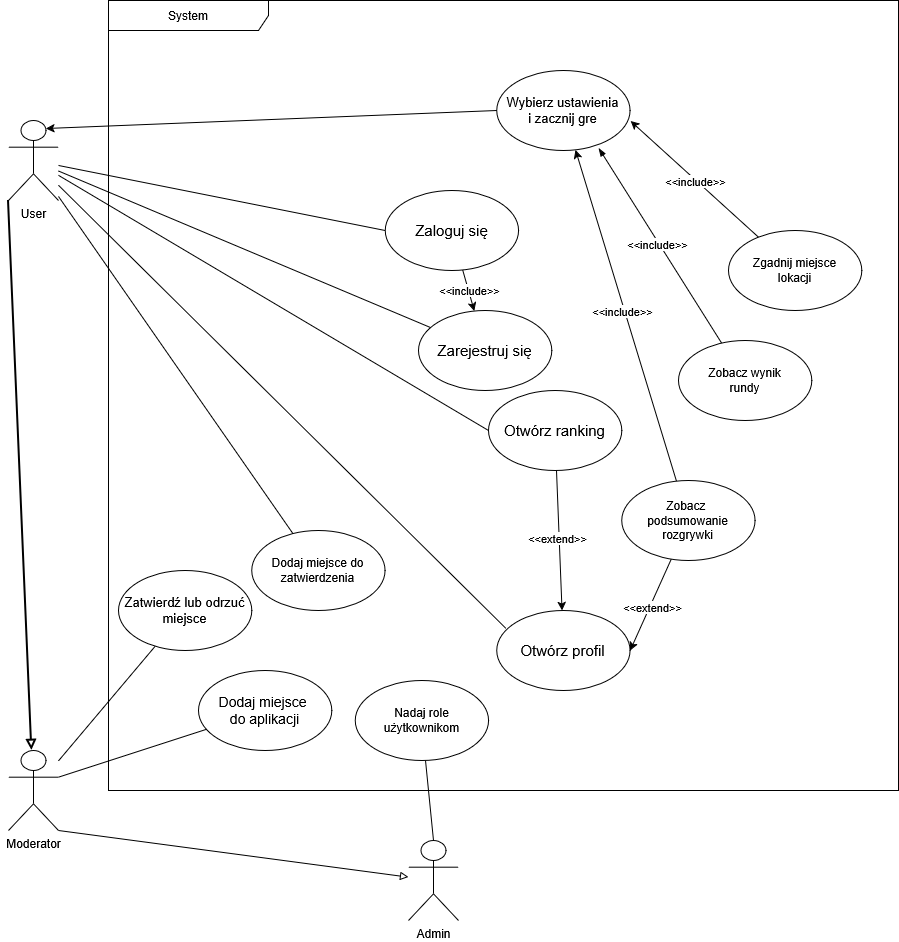
\includegraphics[width=1.0\textwidth]{./images/useCaseDiagram.png}
    \caption{Diagram przypadków użycia aplikacji UniGuesser}
    \label{fig:use-case-diagram}
\end{figure}

\subsection{Diagram sekwencji rozgrywki}

Diagram sekwencji przedstawiony na rysunku \ref{fig:sequence-diagram} ilustruje przebieg interakcji między użytkownikiem a systemem podczas typowej rozgrywki w aplikacji UniGuesser. Proces rozpoczyna się od momentu, gdy użytkownik uruchamia nową grę, poprzez kolejne rundy, aż do momentu zakończenia sesji i wyświetlenia wyników końcowych.

\begin{figure}[H]
    \centering
    \makebox[\textwidth]{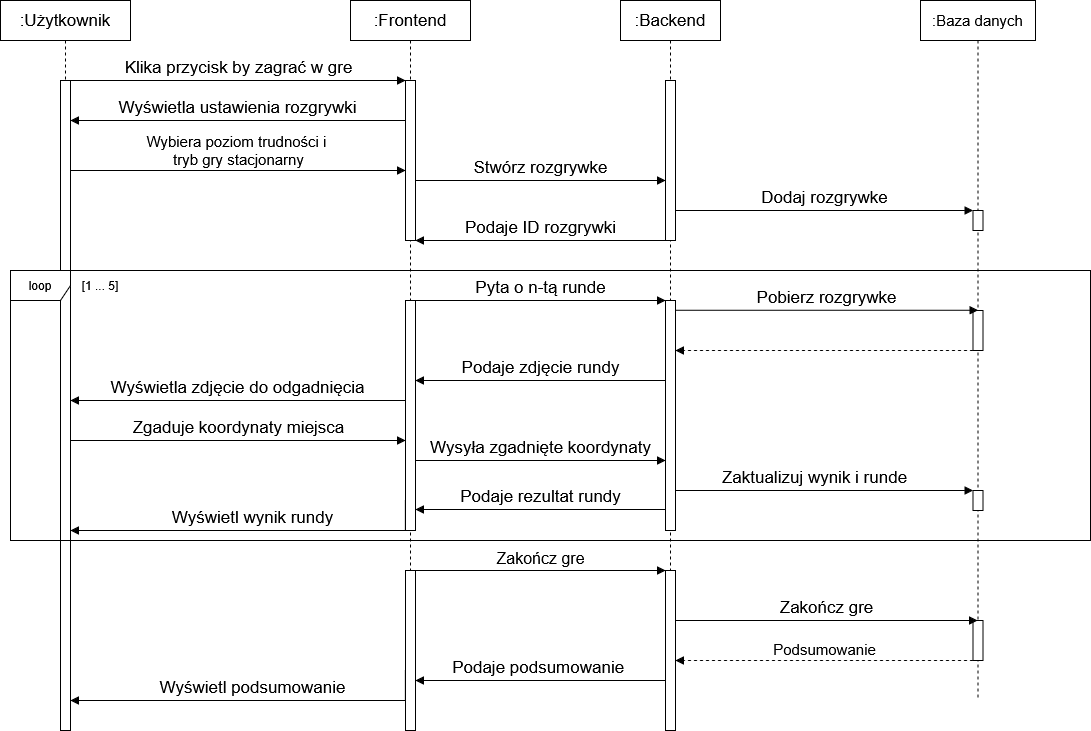
\includegraphics[width=1.2\textwidth]{./images/standardGameplaySequenceDiagram.png}}
    \caption{Diagram sekwencji przedstawiający przebieg rozgrywki w aplikacji UniGuesser}
    \label{fig:sequence-diagram}
\end{figure}

\section{Estetyka i design (Filip Jezierski) }
Wygląd aplikacji został zaprojektowany z myślą o prostocie, intuicyjności oraz atrakcyjności wizualnej. Poniżej przedstawiono kluczowe elementy designu interfejsu użytkownika.

\subsection{Ogólny projekt interfejsu}
Design interfejsu użytkownika naszej aplikacji skupia się na minimalizmie i czytelności. Stosowane są przyjęte jako standardowe układy elementów, takie jak menu nawigacji w górnej części ekranu, co ułatwia poruszanie się po aplikacji, nawet dla nowych użytkowników. Podstrony są zaprojektowane tak, aby unikać nadmiaru informacji, co pozwala użytkownikom skupić się na kluczowych funkcjonalnościach. W trakcie rozgrywki centralnym elementem interfejsu jest interaktywna mapa, która umożliwia użytkownikom łatwe wskazywanie lokalizacji, a pozostałe elementy interfejsu są rozmieszczone w sposób intuicyjny wokół niej.

\subsection{Kolorystyka}
% todo: screen z aplikacji
Aplikacja wykorzystuje dwukolorową paletę barw, opartą na odcieniach białego i ciemnoniebieskiego, inspirowaną kolorystyką Politechniki Gdańskiej. Biały kolor dominuje w tle, co zapewnia czystość i przejrzystość interfejsu, natomiast niebieskie akcenty są używane do wyróżnienia kluczowych elementów, takich jak przyciski, nagłówki czy linki. Przykładowe zastosowanie palety kolorów przedstawia rysunek \ref{fig:register-form}. Taka kolorystyka zapewnia odpowiedni kontrast i ułatwia czytelność tekstu, zwłaszcza przy korzystaniu z aplikacji w różnych warunkach oświetleniowych, co jest szczególnie istotne ze względu na terenowy charakter gry.

\begin{figure}[H]
    \centering
    \makebox[\textwidth]{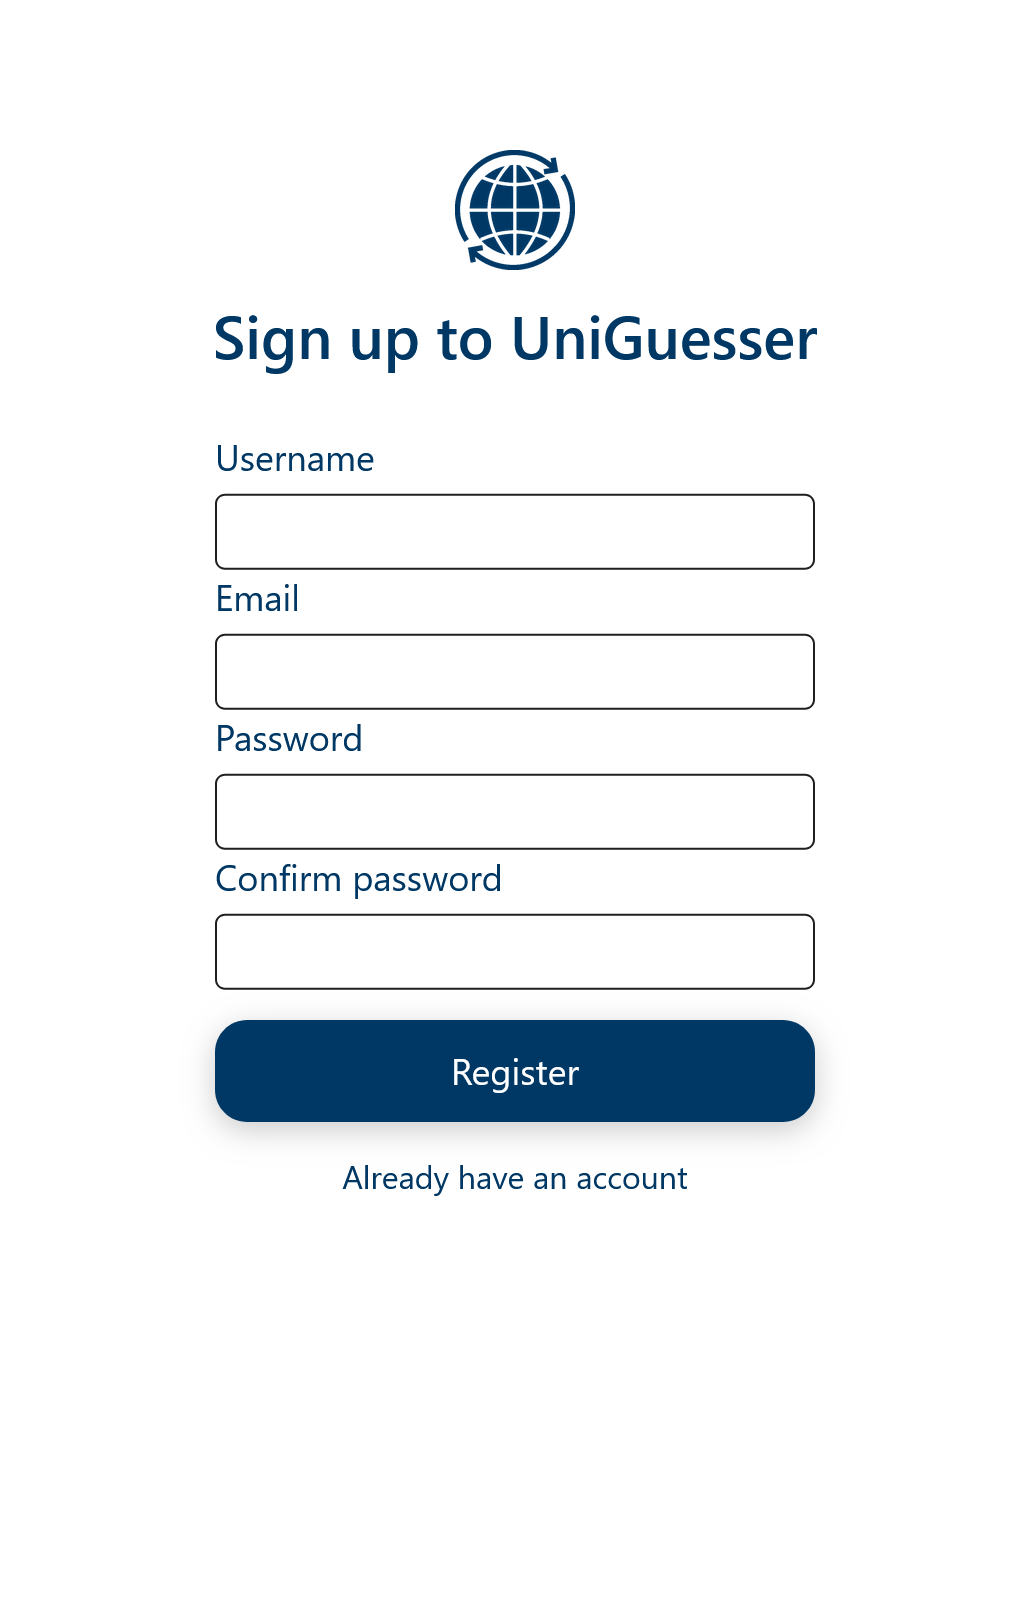
\includegraphics[width=0.5\textwidth]{./images/registerForm.png}}
    \caption{Przykładowy ekran rejestracji użytkownika w aplikacji UniGuesser, ilustrujący zastosowaną kolorystykę}
    \label{fig:register-form}
\end{figure}

\subsection{Typografia}
Aplikacja wykorzystuje czcionkę Roboto, która jest nowoczesna, czytelna i estetyczna. Czcionka ta jest szeroko stosowana w projektach webowych ze względu na swoją uniwersalność i dobrą czytelność na ekranach o różnych rozdzielczościach.

\subsection{Ikony}
W interfejsie użytkownika wykorzystano zestaw prostych i intuicyjnych ikon, pochodzących z biblioteki Google Icons. Ikony te są spójne stylistycznie i pomagają użytkownikom szybko zidentyfikować funkcje oraz akcje dostępne w aplikacji. Dzięki zastosowaniu powszechnie rozpoznawalnych symboli, nawigacja staje się bardziej intuicyjna, co przekłada się na lepsze doświadczenie użytkownika.

\subsection{Responsywność}
Aplikacja została zaprojektowana z myślą o responsywności, co oznacza, że dostosowuje się do różnych rozmiarów ekranów i urządzeń. Dzięki temu użytkownicy mogą korzystać z aplikacji zarówno na komputerach stacjonarnych, jak i urządzeniach mobilnych, bez utraty funkcjonalności czy estetyki. Elementy interfejsu, takie jak przyciski, formularze czy mapy, automatycznie dostosowują swoje rozmiary i układ w zależności od dostępnej przestrzeni ekranowej. Na mniejszych ekranach, takich jak smartfony, menu nawigacyjne jest ukryte za ikoną hamburgera, co pozwala zaoszczędzić miejsce i utrzymać przejrzystość interfejsu. Ponadto, kluczowe funkcje pozostają łatwo dostępne, a tekst i grafiki są skalowane odpowiednio do rozdzielczości ekranu, zapewniając optymalne doświadczenie użytkownika niezależnie od urządzenia.
